\chapter{Introducción}
\label{cap:capitulo1}
\setcounter{page}{1}

\begin{flushright}
\begin{minipage}[]{10cm}
%\emph{Quizás algún fragmento de libro inspirador...}\\
\end{minipage}\\

%Autor, \textit{Título}\\
\end{flushright}

\vspace{1cm}

El desarrollo tecnológico ha provocado el avance en la robótica, un campo de investigación muy amplio en la actualidad que está facilitando la vida a los humanos. Cualquier robot está formado por tres componentes principales: un sistema de control, sensores y actuadores. Dentro de los numerosos sensores que pueden tener los robots, uno de los que está adquiriendo mayor relevancia en los últimos años es el sensor de visión.\\

Los sensores de visión aportan mucha información y son baratos, pero se requiere de un proceso arduo para extraer la información útil en tiempo real. Por este motivo se busca la eficiencia en resultados y tiempo, lo que significa que el proceso de extracción de la información debe ser rápido. Es por ello que en los últimos años, en el campo de la visión artificial moderna, están adquiriendo gran importancia los algoritmos de Deep Learning (DL) o aprendizaje profundo, usados para adquirir esta información.\\

Los algoritmos más utilizados hoy en día para obtener la información de los sensores de Visión Artificial (VA) se obtienen bajo la técnica del Machine Learning (ML) o aprendizaje automático. Estos algoritmos son mejores que los que se tenían anteriormente, y se han podido desarrollar gracias al avance de la capacidad de cómputo. El objetivo del ML es que las máquinas sean capaces de aprender sin tener que ser programadas explícitamente.\\

Un subcampo del ML es el DL, que aunque este segundo utiliza algoritmos del primero, sus algoritmos se basan en estructuras similares al modelo del cerebro humano, emulando redes neuronales. A medida que el algoritmo de DL obtiene más información, aumenta su precisión. Debido a su gran capacidad de abstracción, es el más usado en VA.\\

A continuación se describen estos conceptos y el contexto en el que se enmarca el presente trabajo. Asimismo se presentan sistemas actuales que existen en el mercado con una idea similar a la de este trabajo.\\

\section{La robótica}
\label{sec:robotica}
La robótica, aunque no siempre bajo ese nombre, se lleva utilizando desde hace mucho tiempo con el propósito de desarrollar herramientas automatizadas.
Hasta mediados del siglo pasado, esta disciplina se centraba en el desarrollo de máquinas que realizaban un trabajo que resultaba tedioso, debido a su repetitividad, para el ser humano. Esta concepción se refleja con Henry Ford y la producción en serie de su fábrica de coches inaugurada en 1901 (Figura \ref{fig:ford}).\\
\begin{figure} [h!]
  \begin{center}
    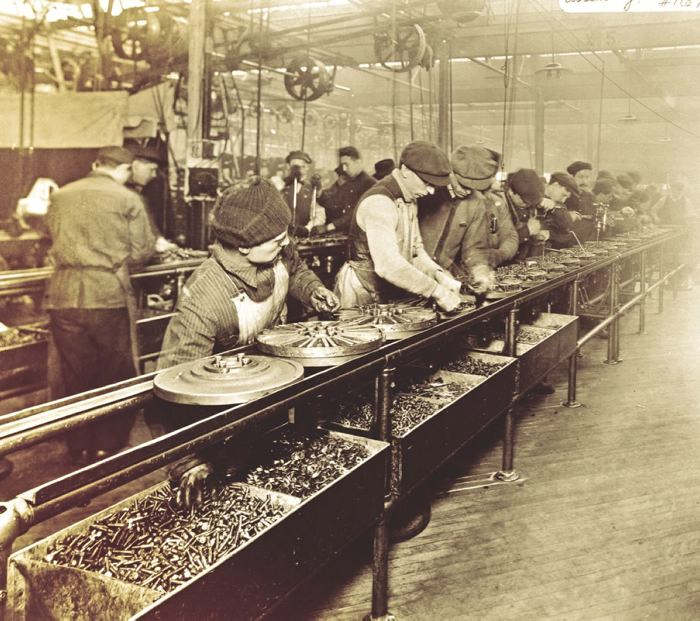
\includegraphics[width=8cm]{figs/ford}
  \end{center}
  \caption{Producción en serie en la fábrica de coches Ford.}
  \label{fig:ford}
\end{figure}

Sin embargo, la palabra \textit{robota} ---origen de la palabra robot que significa trabajo forzado--- aparece por primera vez en 1921 en una obra de teatro de un autor checo llamado Karel Capek. Empezando a concebir esta palabra a principios de siglo pasado, comenzó a nacer el desarrollo de la idea de robótica que existe hoy en día y que no se centra exclusivamente en el desarrollo de herramientas automatizadas, sino que se concibe como una industria interdisciplinaria que surge de la intersección de la ciencia, la ingeniería y la tecnología. Esta nueva concepción une el conocimiento científico, computacional e informático con diversas ramas de la ingeniería, ya que no solo implica el estudio de robots, sino también de su diseño, programación y aplicación. Así, la robótica incluye disciplinas como la IA, la informática, la VA, la programación o el álgebra, entre otras muchas.\\

Tras la primera aparición de la palabra \textit{robota}, la definición de robot ha ido formándose hasta la que hay en la actualidad:  cualquier máquina que opera de forma automática y autónoma, y que sustituye a los seres humanos en determinadas tareas, especialmente las peligrosas, aburridas o pesadas. Está compuesto por el sistema de control, los sensores y los actuadores.\\

La analogía de un robot respecto a un ser humano es la siguiente. Los sensores son sus sentidos, que transmiten la información percibida, bien sea del propio robot o del entorno al sistema de control, que se asemeja al cerebro humano. El sistema de control toma decisiones adaptándose a la información recibida, que modifica bien el entorno o bien la manera de actuar internamente del propio robot. Y finalmente los actuadores, que permiten la modificación del entorno; su equivalente en el cuerpo humano serían las extremidades.\\

El objetivo de la robótica es ayudar al ser humano en todos los ámbitos, tanto en la vida cotidiana como en la vida profesional, evitando los trabajos perjudiciales, e incluso haciendo trabajos que el ser humano no sería capaz de hacer por sí mismo en distintos sectores.\\

Uno de estos sectores es la medicina. En este ámbito cabe resaltar el robot Da Vinci (Figura \ref{fig:da-vinci}), uno de sus robots más famosos que permite a un cirujano comandar órdenes a través de una consola, permitiéndole realizar cirugías de alta precisión eliminando los temblores nerviosos que un humano pueda tener y permitiendo al cirujano una mayor visión. Otro ejemplo en el campo de la medicina se encuentra en la impresión 3D. En \cite{ANDRESCANO2021138}, la impresión 3D de biomodelos de partes del cuerpo (por ejemplo huesos) adquiere un papel útil en fracturas complejas, displasias de cadera o en tumores óseos principalmente. Con estos biomodelos, no solo disminuye tanto el tiempo quirúrgico como los costes de intervención, sino que además se reduce la dosis intraoperatoria de radiación. También sirven para la planificación preoperatoria (Figura \ref{fig:3d}-a) o el premodelado de placas (Figura \ref{fig:3d}-b). Con la impresión 3D también se han creado férulas para los pacientes (Figura \ref{fig:3d}-c), ya que ofrecen una mayor adaptación a la anatomía del paciente que las férulas de yeso o plástico que se acostumbran a llevar.\\
\begin{figure} [h!]
  \begin{center}
    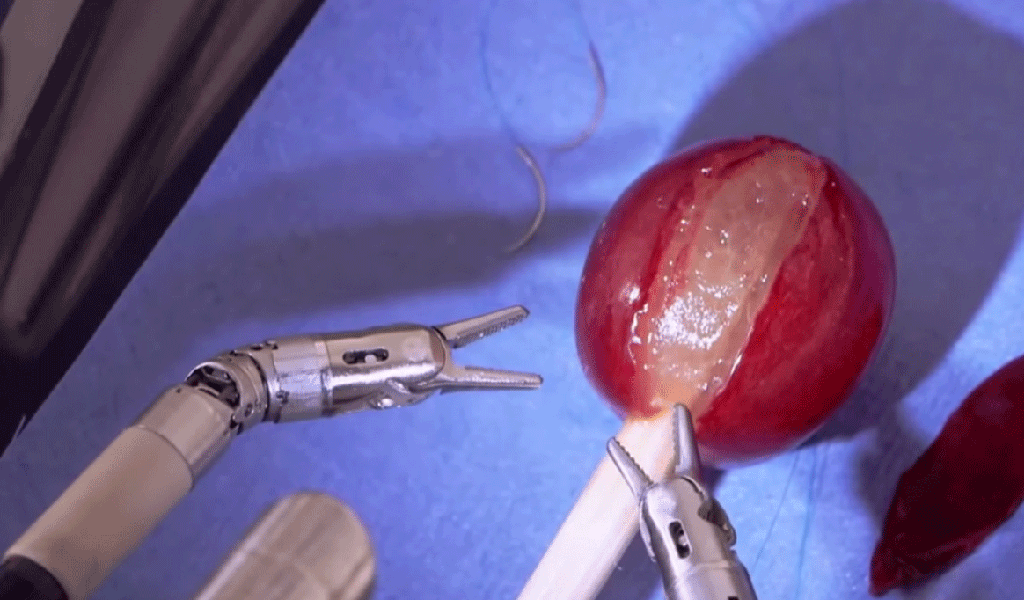
\includegraphics[width=8cm]{figs/da-vinci}
  \end{center}
  \caption{Robot Da Vinci}
  \label{fig:da-vinci}
\end{figure}

\begin{figure}[h!]
  \begin{center}
    \subfigure[Preoperatoria]{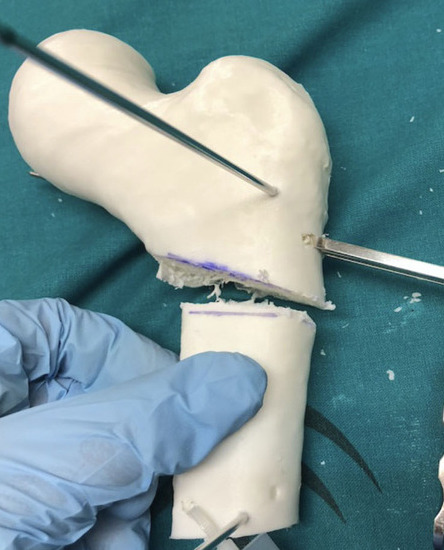
\includegraphics[width=41mm]{figs/preop}}\hspace{2mm}
    \subfigure[Premodelado de placas]{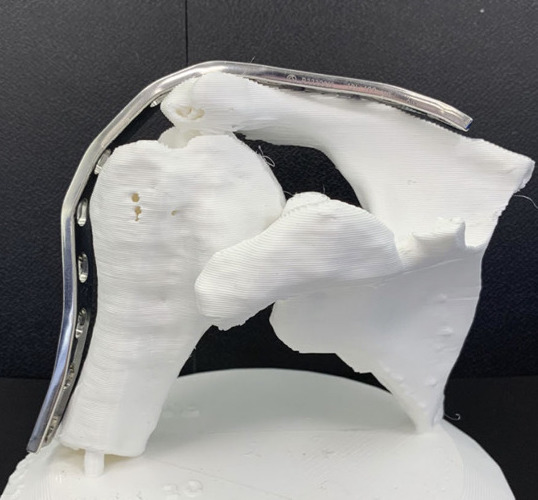
\includegraphics[width=55mm]{figs/premodelado}}
    \subfigure[Férulas con impresión 3D]{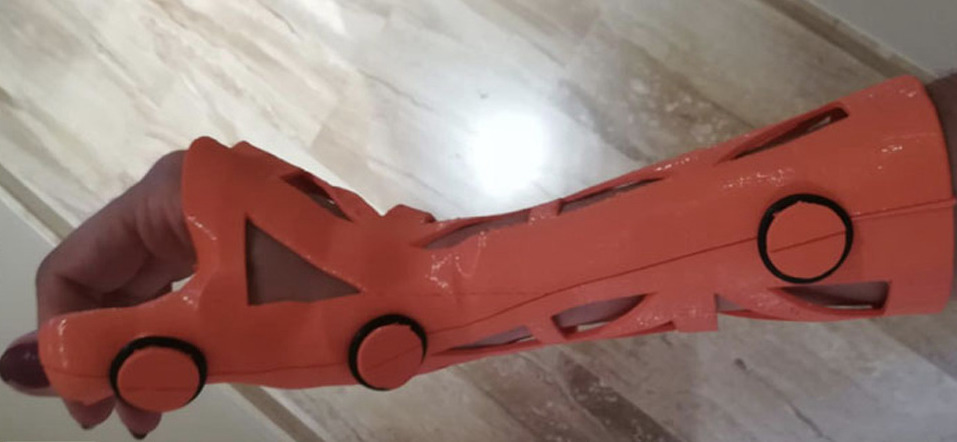
\includegraphics[width=100mm]{figs/ferula}}
  \end{center}
\caption{Usos de la impresión 3D en medicina.} \label{fig:3d}
\end{figure}

Otro de los campos más importantes de la robótica es la manipulación en entornos inaccesibles u hostiles para el ser humano. Un ejemplo de ello lo encontramos en la carrera espacial. Uno de estos robots es el Curiosity (Figura \ref{fig:robots}-a), cuya misión era evaluar la habitabilidad en Marte recogiendo información del entorno. Otro ejemplo de entornos hostiles se encuentra en el lugar que quedó tras el accidente nuclear que ocurrió en Fukushima en 2011, causado por un terremoto y el consecuente tsunami. Gracias a los robots (Figura \ref{fig:robots}-b) se pudo acceder a la zona para poder limpiarla.\\
\begin{figure}[h!]
  \begin{center}
    \subfigure[Robot Curiosity]{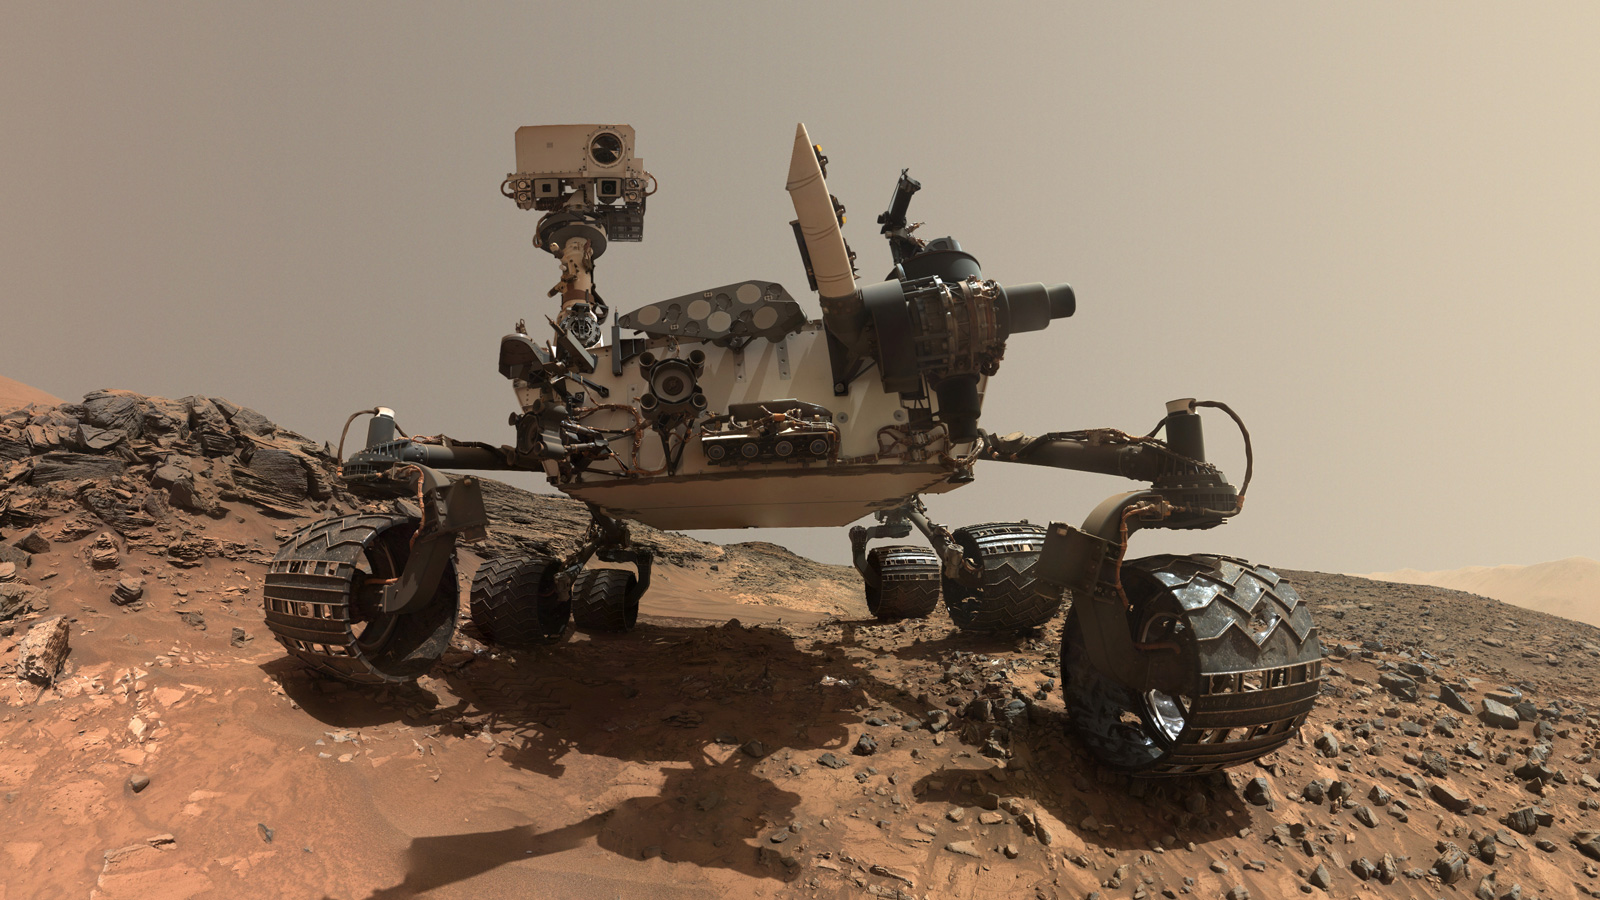
\includegraphics[width=82mm]{figs/curiosity}}\hspace{2mm}
    \subfigure[Robot en Fukushima]{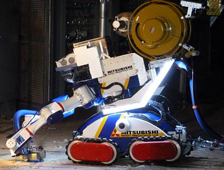
\includegraphics[width=61mm]{figs/fukushima}}
  \end{center}
\caption{Ejemplos de la robótica en diferentes campos.} \label{fig:robots}
\end{figure}

La industria del automóvil, con los coches autónomos (Figura \ref{fig:coches}-a), es otro de los grandes frentes de la robótica. El objetivo es que un coche sea capaz de realizar todas las tareas de conducción de forma autónoma. Como medio autónomo, es capaz de percibir el medio que le rodea y navegar en consecuencia.
\begin{figure}[h!]
  \begin{center}
    \subfigure[Coche autónomo de Google]{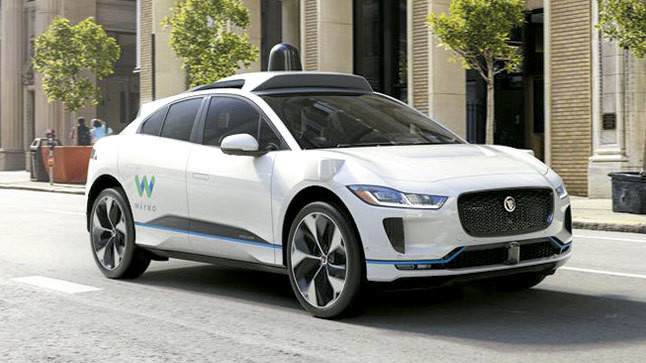
\includegraphics[width=7.5cm]{figs/coche}}
    \subfigure[Vision de un Tesla autónomo]{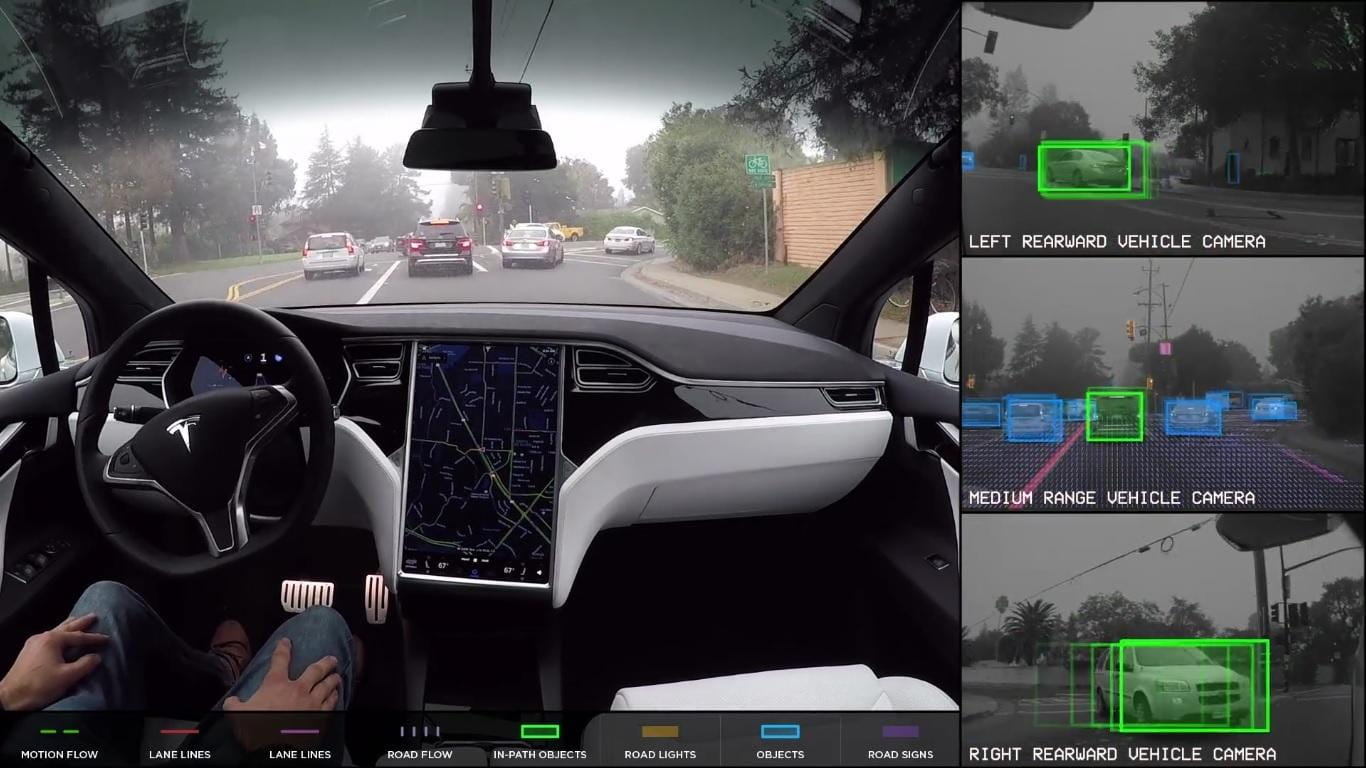
\includegraphics[width=7.5cm]{figs/coche_autonomo}}
  \end{center}
\caption{Ejemplos de la robótica en diferentes campos.} \label{fig:coches}
\end{figure}

\section{Inteligencia Artificial}
La robótica engloba un conjunto de diferentes disciplinas que permiten abordar todos los campos que esta comprende. Uno de los campos más importantes es la Inteligencia Artificial (IA), que consiste en replicar los mecanismos del cerebro humano mediante algoritmos que emplean unidades equivalentes a las neuronas. Estos algoritmos van aprendiendo a medida que realizan sus tareas en base a la experiencia que van adquiriendo durante su ejecución.\\

Numerosos son los estudios existentes en la actualidad sobre la IA. Uno de ellos es la mejora del rendimiento y la eficiencia  del reconocimiento de fracturas radiográficas a través de la IA \cite{guermazi21}. Este algoritmo es capaz de detectar las fracturas en las radiografías con un menor rango de fallo y en menor tiempo que un humano. En el caso de la Figura \ref{fig:rad1}, nueve especialistas no detectaron la fractura mientras que el algoritmo sí.\\
\begin{figure} [h!]
  \begin{center}
    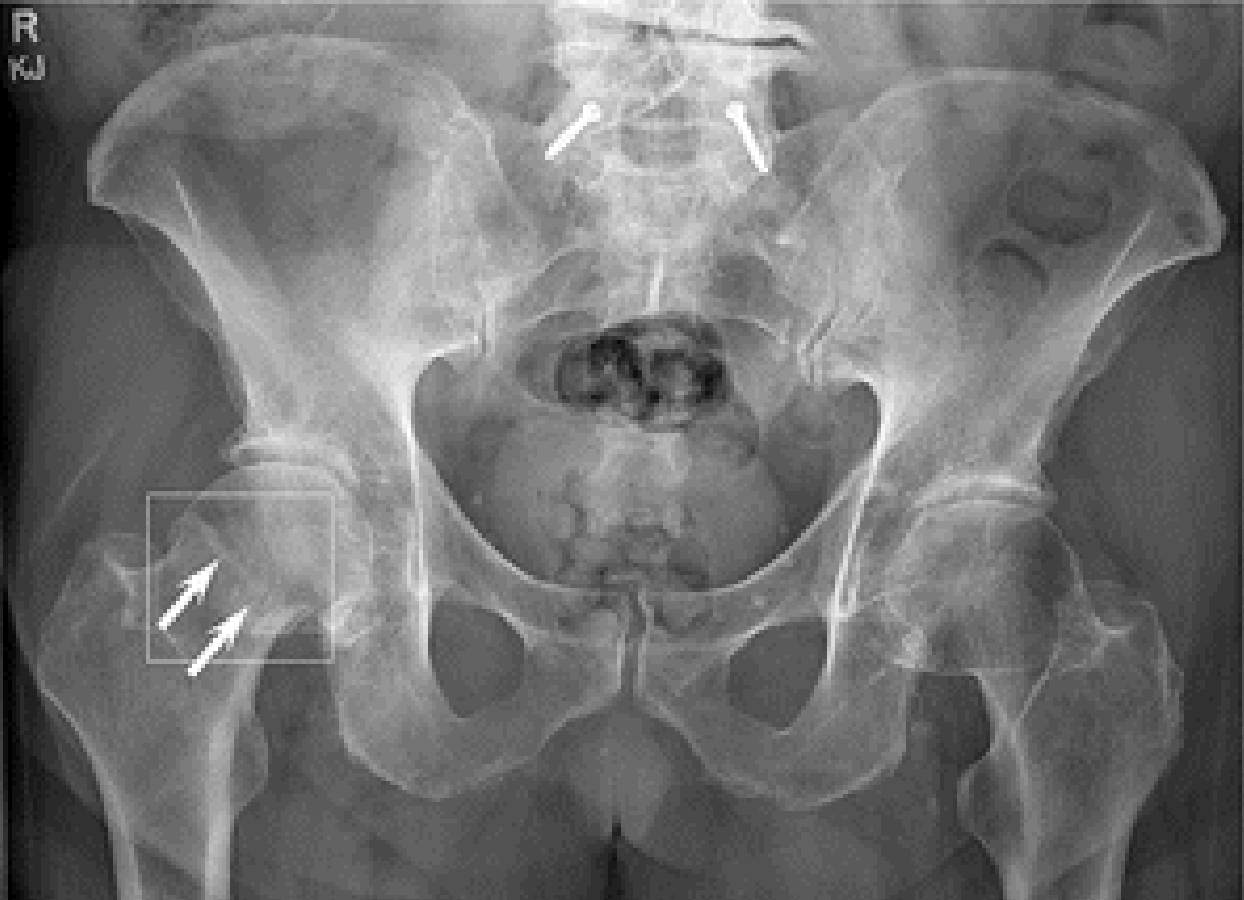
\includegraphics[width=8cm]{figs/rad1}
  \end{center}
  \caption{Detección de fracturas en la radiografía mediante IA}
  \label{fig:rad1}
\end{figure}

Hay dos tipos de inteligencia artificial:
\begin{itemize}
 \item{IA fuerte,} compuesta por la IA general y la superinteligencia artificial. La IA general está inspirada en la teoría de que una máquina adquiera inteligencia humana, siendo capaz de resolver cualquier problema por sí misma. Por otro lado, la superinteligencia artificial supera la capacidad del cerebro humano. La IA fuerte es todavía teórica y no hay ejemplos reales de su uso.
  \item{IA débil,} entrenada para realizar tareas específicas que operan dentro de un rango previamente definido. Los sistemas dotados con esta inteligencia parecen inteligentes, pero están limitados al contexto en el que trabajan. Un ejemplo de ello es el asistente de voz Siri de Apple.
\end{itemize}

La IA abarca diferentes áreas, como la comprensión, el reconocimiento o el aprendizaje. Una de las líneas de investigación dentro de la IA es la VA, que se detalla a continuación.\\

\subsection{Visión Artificial}
\label{sec:subseccion}
La visión artificial es uno de los campos más importantes de la IA cuyo objetivo es que un sistema inteligente obtenga la información en tiempo real más relevante de las imágenes que percibe. Así como la IA trata de emular un cerebro humano, la VA hace lo mismo con respecto a la visión humana, con la diferencia de que esta segunda cuenta con las experiencias aprendidas para, entre otras cosas, diferenciar los elementos que le rodean, su movimiento, distancia o tamaño. Así pues, la VA trata de asemejar el funcionamiento del ojo humano y su posterior procesamiento con el cerebro mediante  una cámara y el posterior procesamiento de los datos que esta vierte.\\

Tiene diferentes usos, entre ellos los más fundamentales son:
\begin{itemize}
 \item \textit{Clasificación de imágenes (Figura \ref{fig:vision}-a).} Consiste en asignar imágenes a una serie de categorías predefinidas a través de un algoritmo. Es necesario contar con una gran cantidad de datos para poder tener suficiente entrenamiento y así fallar lo mínimo posible.
 \item \textit{Detección de objetos (Figura \ref{fig:vision}-b).} Consiste en analizar partes de la imagen para localizar objetos señalándolos mediante cuadros limitadores. Esto se consigue mediante el entrenamiento de una gran cantidad de imágenes en las que se etiquetan diferentes tipos de objetos, obteniendo así los datos que se usarán para la detección en una imagen.
  \item \textit{Segmentación de imágenes(Figura \ref{fig:vision}-c).} Consiste en el enmascaramiento exacto de los píxeles que representan a los objetos en una imagen. Es un paso más en la detección de objetos, siendo capaz de separar el objeto concreto del resto de la imagen. 
\end{itemize}
\begin{figure}[h!]
  \begin{center}
    \subfigure[Clasificación]{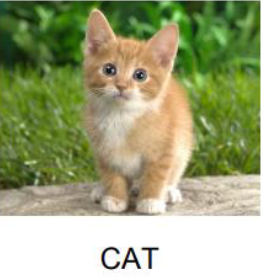
\includegraphics[width=43mm]{figs/clasificacion}}\hspace{8mm}
    \subfigure[Detección]{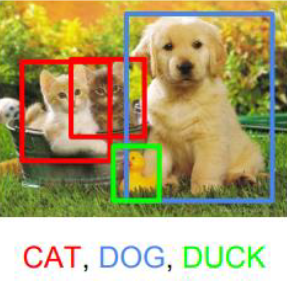
\includegraphics[width=45mm]{figs/deteccion}}\hspace{8mm}
    \subfigure[Segmentación]{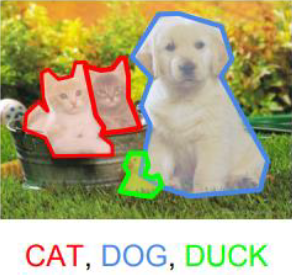
\includegraphics[width=47mm]{figs/segmentacion}}
  \end{center}
\caption{Algunos usos en la visión artificial.} \label{fig:vision}
\end{figure}

Un sistema dotado de VA funciona siguiendo tres niveles de operación. En primer lugar, la obtención de imágenes o vídeos mediante una cámara, las cuales son transferidas al sistema. En segundo lugar, el procesamiento de estas imágenes para poder representar correctamente los datos de interés. Este proceso consiste en un trabajo automático del sistema en el que se elimina el ruido, se reescalan las imágenes o se ajusta el contraste, entre otros, para adaptar las imágenes. Finalmente, se realiza la comprensión de imágenes, que es el paso clave para que el sistema pueda llamarse inteligente, donde a través de un modelo de aprendizaje, es capaz de llevar a cabo su propósito, como puede ser detectar un determinado objeto utilizando datos aprendidos en el pasado.\\

Un ejemplo muy extendido de uso de la VA son los coches autónomos (Figura \ref{fig:coches}-b). En este caso, el funcionamiento de la VA ha de ser impecable debido a las graves consecuencias que supondría el más mínimo fallo. Con el uso de cámaras y sensores, el ordenador del coche es capaz de detectar los objetos de las imágenes que recibe, como señales o semáforos ---entre otros--- y actuar en consecuencia según el estado de estos. Así, el coche es capaz de tener una vista de 360º y de reconocer todos los elementos de su entorno para ser capaz de actuar como lo haría un humano.\\

Para que la VA funcione correctamente es necesario disponer de algoritmos precisos que sean fiables. Entre los distintos métodos que existen para entrenar estos algoritmos, uno de los más utilizados es el ML, que se detalla a continuación.

\section{Machine Learning}
Para que la IA pueda simular al cerebro humano, debe ser capaz también de aprender. Este aprendizaje se lleva a cabo a través de algoritmos. Dentro de la IA se encuentra una categoría denominada Machine Learning o aprendizaje automático, cuyo fin es que los algoritmos descubran patrones en conjuntos de datos que les hacen aprender y mejorar respecto a la experiencia anterior pudiendo así tener un aprendizaje autónomo para poder realizar una tarea sin ayuda externa.\\

En el sistema de aprendizaje de un algoritmo de ML hay tres partes principales. En primer lugar, un proceso de decisión, en el que una vez recibidos los datos de entrada el algoritmo genera una estimación en los datos partiendo de un patrón. Los datos de entrada pueden estar o no etiquetados; si lo están, indican al modelo lo que debe identificar. La segunda parte es una función de error, que sirve para evaluar la precisión del modelo sobre la decisión tomada. La tercera y última parte es un proceso de optimización de modelos donde las ponderaciones se ajustan en el caso de que el modelo se pueda adaptar mejor al conjunto de datos de entrenamiento, repitiendo este proceso hasta cumplir un umbral de precisión.\\

Hay diferentes tipos de \textit{Machine Learning}:
\begin{itemize}
 \item \textit{Aprendizaje supervisado,} donde los conjuntos de datos están etiquetados. Estos conjuntos de datos sirven para entrenar los datos que servirán como experiencia y base al algoritmo a la hora de hacer una clasificación con un nuevo dato. Por tanto, usa un conjunto de datos entrenados iniciales a la hora de recibir un nuevo dato.
 \item \textit{Aprendizaje no supervisado,} donde los conjuntos de datos están sin etiquetar, es decir, no cuenta con un conjunto entrenado previamente.
 \item \textit{Aprendizaje semisupervisado,} que es el término medio entre los dos anteriores. En este caso, en el entrenamiento se usa un conjunto de datos más pequeño que en el aprendizaje supervisado y usa un grupo más grande de datos sin etiquetar.
\end{itemize}

\section{Deep Learning}
De la misma forma que el ML está dentro del amplio campo de la IA, el ML también tiene diferentes campos. Entre ellos está el DL (Figura \ref{fig:ia-ml-dl}). Mientras en el ML el autómata está preprogramado por un humano, en el DL el autómata aprende por sí mismo, siendo un ápice más de cómo el DL trata de simular el cerebro humano. Lo hace mediante unidades equivalentes a las neuronas.\\
\begin{figure} [h!]
  \begin{center}
    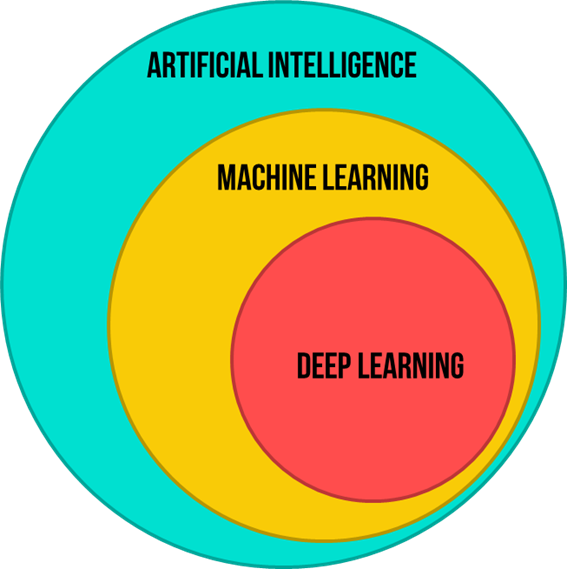
\includegraphics[width=8cm]{figs/ia-ml-dl}
  \end{center}
  \caption{Esquema de relaciones entre IA, ML y DL.}
  \label{fig:ia-ml-dl}
\end{figure}

Mientras el ML necesitaba un humano para definir previamente las características de un conjunto de datos para su clasificación, el Deep Learning no necesita intervención humana. Este aprendizaje profundo se asemeja mucho más al aprendizaje humano por tener un funcionamiento similar al de las neuronas. Este funcionamiento se denomina red neuronal.\\

Las redes neuronales (Figura \ref{fig:red}) están formadas por distintas capas de nodos interconectados, donde cada nodo se basa en su capa anterior para refinar y optimizar la precisión. Está compuesto por la capa visible, que es la primera capa, donde el modelo recibe los nuevos datos de entrada. Las otras son las capas ocultas o \textit{hidden layers}, que son las que realizan todo el proceso de optimización hasta llegar al resultado final.\\
\begin{figure} [h!]
  \begin{center}
    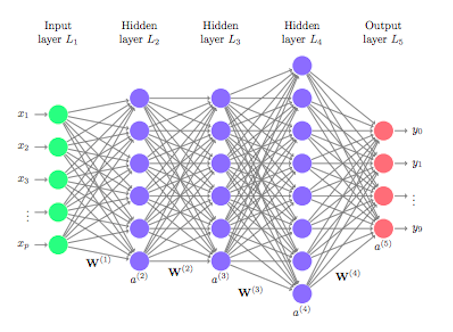
\includegraphics[width=12cm]{figs/deep_learning}
  \end{center}
  \caption{Simple ejemplo de una red neuronal en el algoritmo de Deep Learning.}
  \label{fig:red}
\end{figure}

Existen multitud de estudios sobre el Deep Learning. Uno de ellos ha sido la restauración de textos antiguos con el uso de una red neuronal profunda llamada Ithaca \cite{assael22} (Figura \ref{fig:textos}). Con ella se ha conseguido reparar textos dañados con una precisión del 62\% por sí sola. Está pensada para utilizarla con los historiadores, que han mejorado su precisión del 25\% al 72\% con esta nueva herramienta.\\
\begin{figure} [h!]
  \begin{center}
    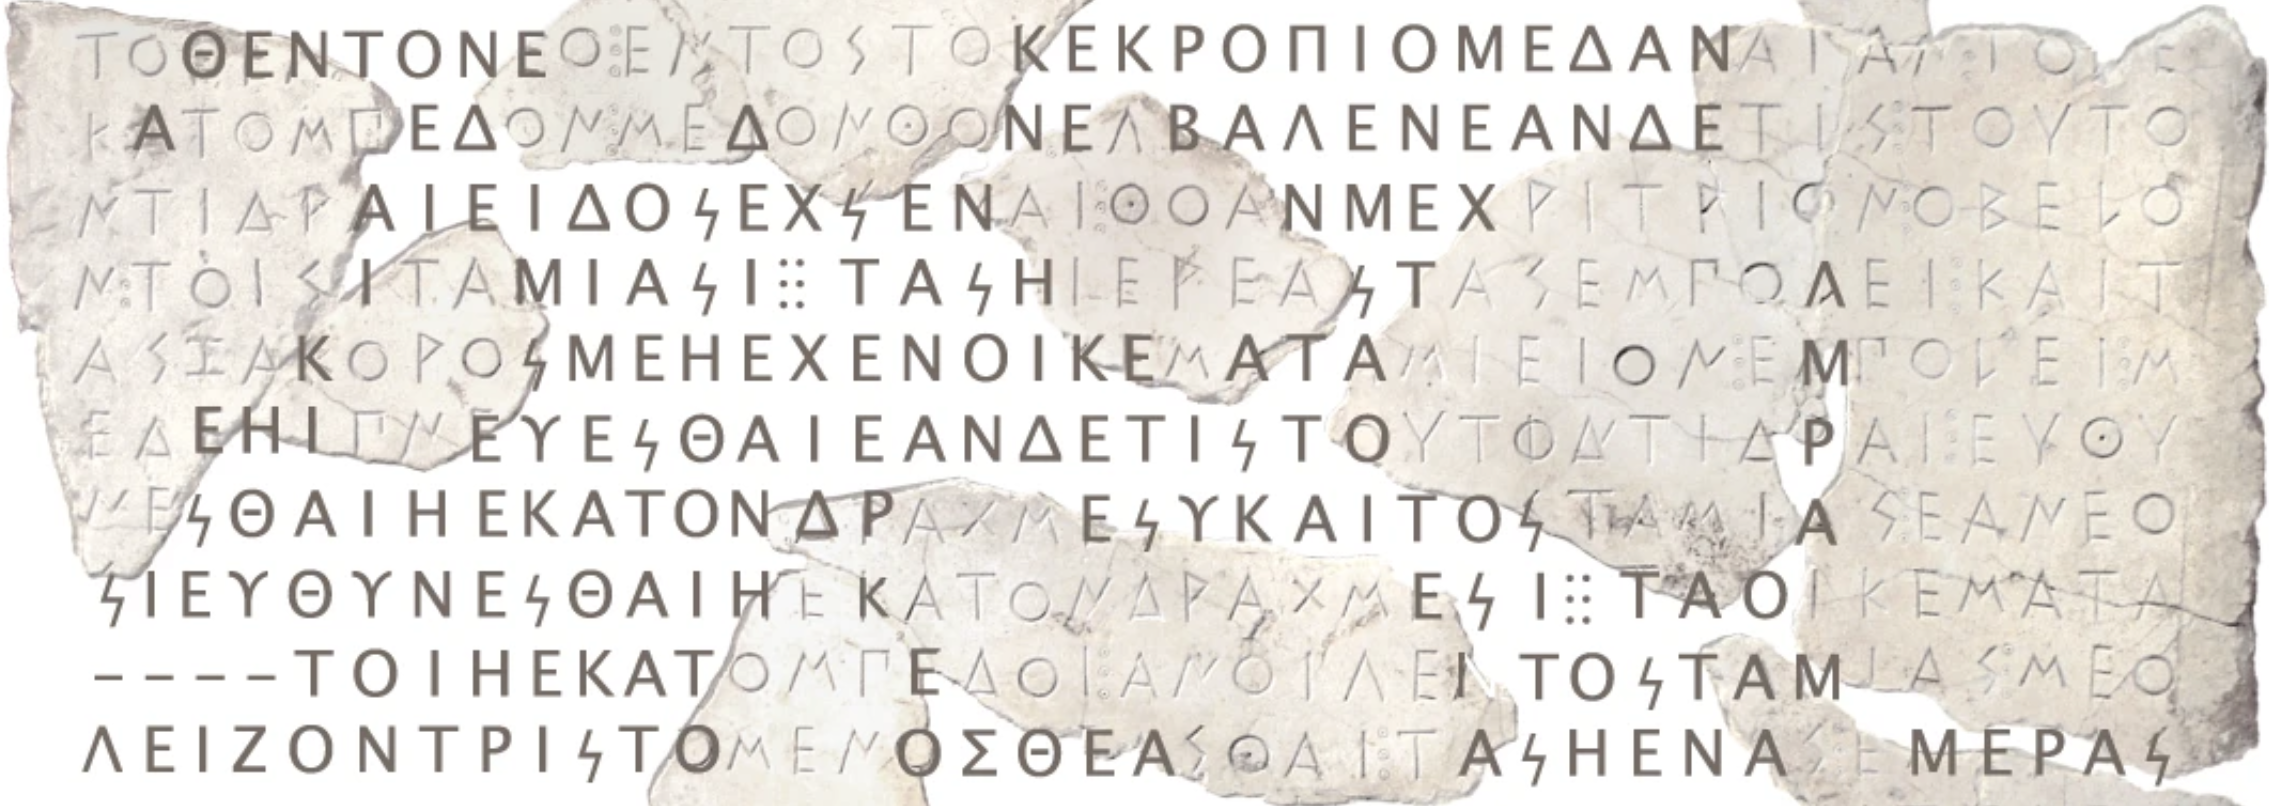
\includegraphics[width=11cm]{figs/textos}
  \end{center}
  \caption{Decreto sobre la Acrópolis de Atenas reconstruido con Ithaca.}
  \label{fig:textos}
\end{figure}

También existen aplicaciones de Deep Learning que se utilizan en la vida cotidiana, como los asistentes virtuales.  Este es el caso de los dispositivos Siri o Alexa ---entre otros--- que, mediante algoritmos de Deep Learning, ayudan a los usuarios a realizar distintas tareas, aprendiendo continuamente de la información que reciben.\\

Otro ejemplo donde se emplean algoritmos de DL es el reconocimiento de imágenes. Aquí se pueden encontrar numerosas aplicaciones prácticas, como por ejemplo el enfoque automático en las caras al realizar fotos (Figura \ref{fig:caras}).\\
\begin{figure} [h!]
  \begin{center}
    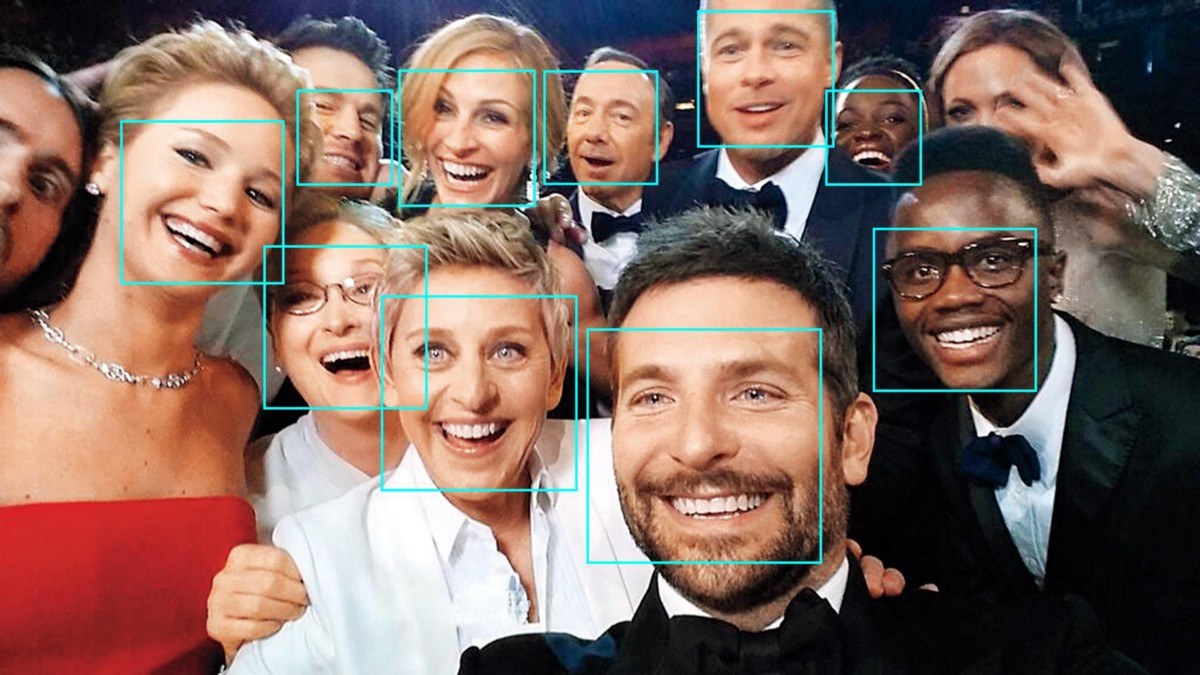
\includegraphics[width=8cm]{figs/caras}
  \end{center}
  \caption{Reconocimiento facial con técnica de Deep Learning.}
  \label{fig:caras}
\end{figure}

\section{Sistemas multisensoriales}
Como se ha explicado en las secciones anteriores, el desarrollo del DL es muy importante. Lo es especialmente en el campo de la VA, pues permite crear aplicaciones sofisticadas que simulan la visión humana. Pero si además del sensor de visión se incorporan otros tipos de sensores a un robot, el resultado de la actuación de este mejora, ya que, además de percibir la imagen del entorno, está percibiendo más información que puede ser útil a la hora de tomar decisiones. Retomando la analogía con el ser humano, si este, además de ver, es capaz de sentir, oler o tocar, recibe más información de su entorno, por lo que puede conocer mejor la situación en la que se encuentra y, con ello, actuar más inteligentemente.\\

Numerosas son las aplicaciones de un sistema multisensorial, por ejemplo para los sistemas propioceptivos. Estos sistemas necesitan conocer con exactitud las variables del entorno. Otra aplicación se encuentra en los robots móviles. Al disponer de múltiples sensores, estos robots reducen el error en sus movimientos o en su autolocalización. Otro ejemplo del uso de sistemas multisensoriales es el seguimiento continuado de animales. Algunos ejemplos de estos sistemas se describen a continuación.\\

En \cite{ucm}, de la Universidad Complutense de Madrid se describe un sistema para detectar de forma temprana las enfermedades o infecciones en animales de granja, más concretamente en cerdos. Este sistema parte de la instalación de microchips y otro tipo de sensores en los animales para poder controlar las condiciones, como su temperatura o el consumo de agua de los bebederos, de forma que un ordenador muestra esta información de manera gráfica. También se incluye una monitorización grupal mediante grabaciones diarias para que el sistema detecte cualquier tipo de actividad no común (Figura \ref{fig:ucm}).\\
\begin{figure} [h!]
  \begin{center}
    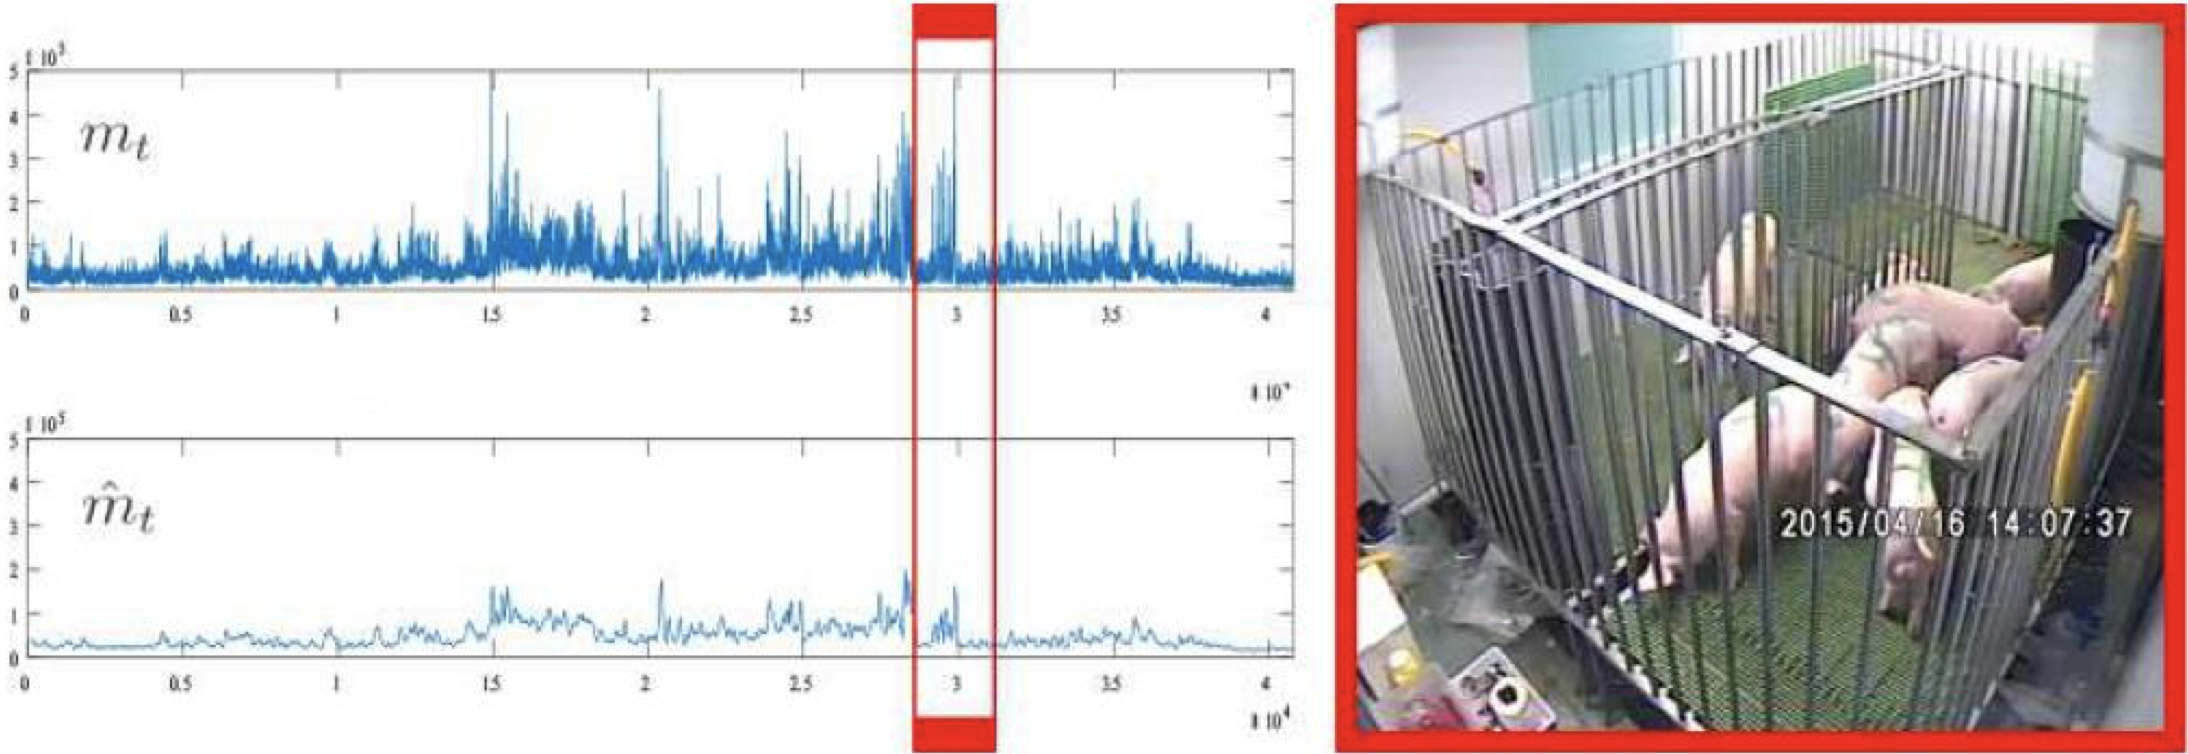
\includegraphics[width=14cm]{figs/ucm}
  \end{center}
  \caption{Patrón de movimientos e imagen grabada del grupo de cerdos.}
  \label{fig:ucm}
\end{figure}

En \cite{arce09}, la Facultad de Zootecnia e Ingeniería de la Universidad de São Paulo presenta un sistema de sensores con el fin de obtener datos fisiológicos de los animales (en este caso vacas) y obtener las condiciones en las que estos tienen menos perturbaciones en su comportamiento natural, pues las condiciones climatológicas en cada región pueden afectar de diferentes maneras: estrés, pérdidas productivas o incluso la muerte. Este sistema se creó con la instalación de sensores en cada una de las vacas creando una red de sensores (Figura \ref{fig:saopaulo}) que se comunican con una estación para obtener todos los datos del conjunto de animales.\\
\begin{figure} [h!]
  \begin{center}
    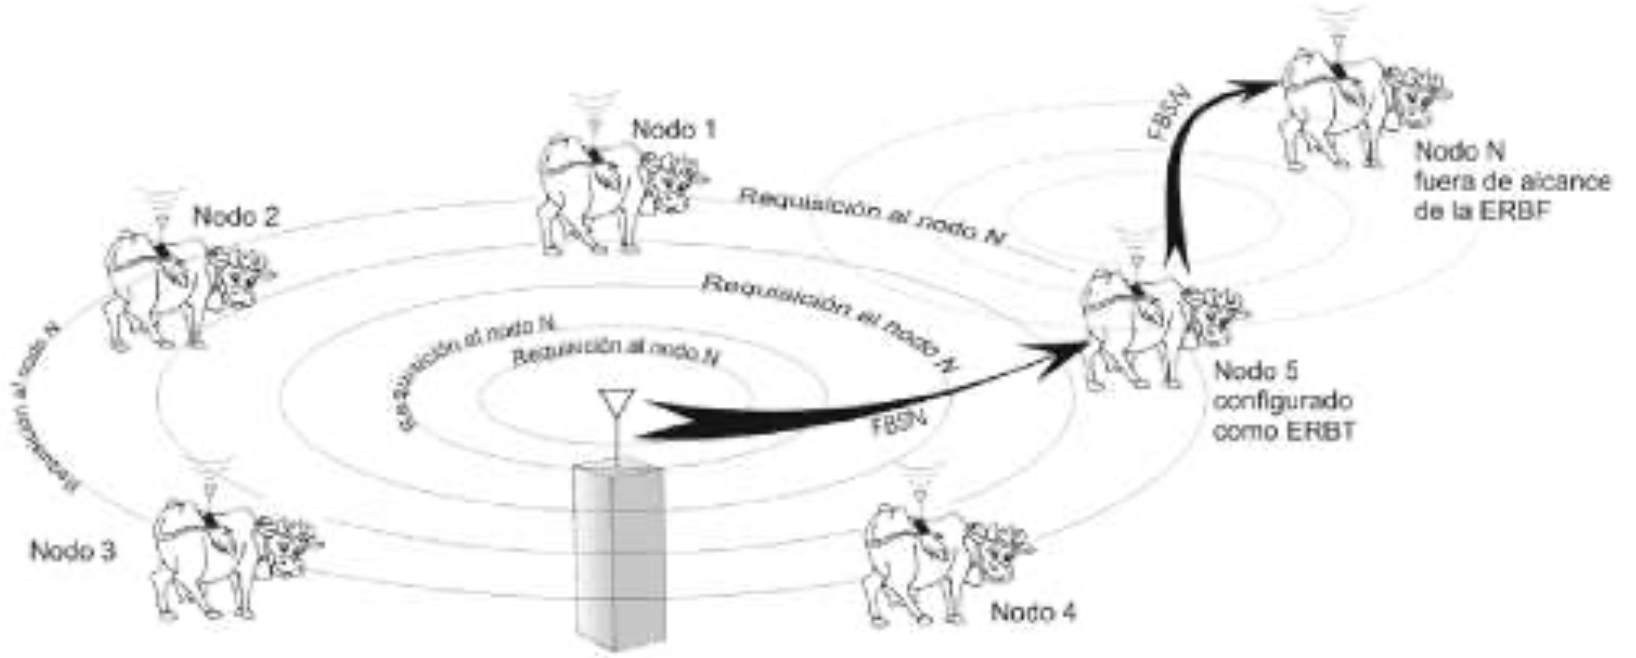
\includegraphics[width=14cm]{figs/saopaulo}
  \end{center}
  \caption{Esquema del desarrollo del sistema mediante sensores.}
  \label{fig:saopaulo}
\end{figure}

El comportamiento que tienen los animales puede ofrecer mucha información acerca de su salud si se mantiene una observación constante, pero también tienen una gran importancia las condiciones del entorno en la que se encuentran, ya que pueden ser decisivas para detectar el motivo de su comportamiento. Por ello, es importante tener un seguimiento constante y automatizado de estas características, permitiendo al humano encargarse únicamente de controlar los datos que el sistema registra.\\
\

\

\

\

\

\
El presente trabajo se enmarca en el contexto de los sistemas multisensoriales, concretamente en los sistemas multisensoriales destinados al bienestar animal y al análisis de comportamiento, en el cual juega un papel fundamental las técnicas de DL.\\

En los próximos capítulos se describe el sistema desarrollado. En el Capítulo 2 se comentan los objetivos, requisitos y metodología del trabajo. En el Capítulo 3 se explican las plataformas de desarrollo que se han utilizado para desarrollar el trabajo. En el Capítulo 4 se describe el proceso exhaustivo que ha llevado el trabajo y finalmente, en el Capítulo 5 se escriben las conclusiones.